
%----------------------------------------------------------------------------------------
%	PACKAGES AND OTHER DOCUMENT CONFIGURATIONS
%----------------------------------------------------------------------------------------

\documentclass{article}

\usepackage{fancyhdr} % Required for custom headers
\usepackage{lastpage} % Required to determine the last page for the footer
\usepackage{extramarks} % Required for headers and footers
\usepackage{graphicx} % Required to insert images
\usepackage{lipsum} % Used for inserting dummy 'Lorem ipsum' text into the template
\usepackage{amsmath}
\usepackage{amsthm}
\usepackage{listings}
\usepackage{xcolor}


\definecolor{grey}{gray}{0.9}
\definecolor{apricot}{rgb}{0.98, 0.81, 0.69}
\definecolor{antiquewhite}{rgb}{0.98, 0.92, 0.84}
\definecolor{bananamania}{rgb}{0.98, 0.91, 0.71}
\definecolor{beige}{rgb}{0.96, 0.96, 0.86}
\definecolor{cream}{rgb}{1.0, 0.99, 0.82}

\lstset{frame=single, basicstyle=\color{black}\ttfamily, backgroundcolor=\color{cream}}

%\lstdefinelanguage{args}{
%sensitive=false,
%alsoletter={.},
%moredelim=[s][\color{red}]{<}{>},
%moredelim=[s][\color{blue}]{[}{]},
%moredelim=[is][\color{orange}]{:}{:},
%keywords=[10]{...},
%keywordstyle=[10]{\color{magenta}},
%}

\lstnewenvironment{arguments}
{\lstset{language=args}}
{}

\lstnewenvironment{bash}
{\lstset{backgroundcolor=\color{white},numbers=left,language=bash,keywordstyle={\color{blue}},frame=single}}
{}



\newtheorem{example}{Example}
\newtheorem*{example*}{Example}
\newtheorem{theorem}{Theorem}
\newtheorem*{theorem*}{Theorem}


% Margins
\topmargin=-0.45in
\evensidemargin=0in
\oddsidemargin=0in
\textwidth=6.5in
\textheight=9.0in
\headsep=0.25in 

% Line spacing
\linespread{1.1}

% Header and footer setup
\pagestyle{fancy}
\lhead{Introduction to the Command Line and Git} % Top left header
\chead{} % Top center header
\rhead{Hautahi Kingi} % Top right header
\lfoot{} % Bottom left footer
\cfoot{} % Bottom center footer

%\rfoot{Page\ \thepage\ of\ \pageref{LastPage}} % Bottom right footer
\renewcommand\headrulewidth{0.4pt} % Size of the header rule
\renewcommand\footrulewidth{0.4pt} % Size of the footer rule

\setlength\parindent{0pt} % Removes all indentation from paragraphs

%----------------------------------------------------------------------------------------
%	NAME AND CLASS SECTION
%----------------------------------------------------------------------------------------

\newcommand{\hmwkTitle}{Problem Set 1} % Assignment title
\newcommand{\hmwkDueDate}{Monday,\ January\ 1,\ 2012} % Due date
\newcommand{\hmwkClass}{} % Course/class
\newcommand{\hmwkClassTime}{10.20} % Class/lecture time
\newcommand{\hmwkClassInstructor}{Hi} % Teacher/lecturer
\newcommand{\hmwkAuthorName}{Hautahi Kingi} % Your name

%----------------------------------------------------------------------------------------
%	TITLE PAGE SETUP
%----------------------------------------------------------------------------------------

\title{
\vspace{2in}
\textmd{\textbf{A Brief Introduction to the Command Line and Git}}\\
\normalsize\vspace{0.1in}\small{Hautahi Kingi}\\
%\vspace{0.1in}\large{\textit{Italic Subtitle}}
\vspace{0in}
}
%\author{\textbf{Bottom Title}}
\date{} %

%
%The source for figure 1: http://acad.coloradocollege.edu/dept/pc/SciCompLab/UnixTutorial/tree.gif

%----------------------------------------------------------------------------------------
\AtBeginDocument{\renewcommand{\abstractname}{}}
\begin{document}

\maketitle

\begin{abstract}
Most of this material was taken from the Software Carpentry website and their excellent bootcamp. More detailed explanations of what I discuss in these notes can be found at: http://software-carpentry.org/lessons.html
\end{abstract}

%----------------------------------------------------------------------------------------
%	TEXT
%----------------------------------------------------------------------------------------

\newpage

\section{What you need}

\begin{enumerate}
\item
Git and the bash shell: For windows users, go to https://msysgit.googlecode.com/files/Git-1.8.4-preview20130916.exe. This will provide you with both Git and Bash in the Git Bash program. For Mac users the bash shell is already installed, so go to http://git-scm.com/downloads to download Git.
\item
An account at GitHub: https://github.com/
\item
The GitHub GUI: https://mac.github.com/ or https://windows.github.com/
\item
A text editor, although this shouldn't be a problem as the default text editor will do nicely (Nano on Mac and Notepad on Windows.)
\end{enumerate}



\section{The Shell and Terminal}

We can interact with a computer in many different ways. Most of us use windows, icons and mice. But these technologies didn't become widespread until the 1980s. Before this, computer users interacted using command-line interfaces as opposed to the graphical user interfaces (GUIs) that are so common today. While GUIs allow for easier and more intuitive navigation of an operating system and its most common tasks (word processing, email, moving files etc.), command-line operations can be very powerful tools when we would like to perform more complex tasks.\\

Let's first address the confusing jargon. You will often hear terms line \emph{command-line interface}, \emph{kernel}, \emph{console}, \emph{command prompt}, \emph{command shell}, \emph{terminal}, \emph{terminal emulator} etc. being used interchangeably. There is a historical reason for each separate term but nowadays the distinction between each is blurred and many have become synonymous with each other. For now, let's stick with \textbf{shell} and \textbf{terminal}, which have a clear distinction.\\

A \textbf{shell} is a computer program like any other. But its primary purpose is to read commands and run other programs, rather than to perform tasks/calculations itself. The most popular shell is Bash. Bash is the default shell on most modern implementations of the Unix operating system (such as Linux and Mac OS X), and in most packages that provide Unix-like tools for Windows.\\

We interact with the shell through a command-line interface or \textbf{terminal}. We do so by entering commands as text input and then pressing enter. The terminal reads the text input, interprets the commands and sends instructions to the shell, which then executes the appropriate operating system functions. Once the commands are carried out, the shell communicates this with the terminal which then prints its output. We then type another command, and so on until the user logs off. This structure is often referred to as REPL (read-evaluate-print loop).\\

Using a shell feels like programming and can be intimidating for beginners. Users are required to know the names of the commands and the syntax of the language that is interpreted. Commands are often only a couple of characters long, their names are frequently cryptic, and their output is lines of text rather than something visual like a graph. However, the shell allows us to combine existing tools in powerful ways with only a few keystrokes. In addition, the command line is often the easiest way to interact with remote machines. As clusters and cloud computing become more popular for scientific data crunching, being able to drive them is becoming a necessary skill.


%%%%%%%%%%%%%%%%%%%%%%%%%%%%%%%%%%%%%%
\newpage
\section{Getting started with the Terminal}


The \textbf{command prompt} is a sequence of one or more characters in the terminal to indicate its readiness to accept commands. The command prompt can vary between machines, but usually ends with a \textbf{\$} or \textbf{\%} character. Experienced users find it useful to customize the command  prompt, but we'll stick with the default here.\\

To begin, type \emph{whoami} into the terminal.
\begin{lstlisting}
$ whoami
hautahikingi
$ 
\end{lstlisting}
The command's output is the ID of the current user. When we type \emph{whoami}, the shell finds a program called whoami, runs that program, displays that program's output (your username), then displays a new prompt to tell us that it is ready for more commands.\\

Now let's try the following.
\begin{lstlisting}
$ pwd
/Users/hautahikingi
\end{lstlisting}
This stands for \emph{print working directory}. When you first login, your current working directory is your home directory. Your home directory has the same name as your username, and it is where your personal files and subdirectories are saved.\\

To find out what is in your home directory, type
\begin{lstlisting}
$ ls				
Desktop		Dropbox		Pictures
Documents	essay.txt	
Downloads	Movies
\end{lstlisting}
\emph{ls} prints the names of the files and directories in the current directory in alphabetical order, arranged neatly into columns.\\

A number of commands have extra options or features which we can call through the use of a \textbf{flag}. A flag is usually a dash followed by a single letter, such as -v. For example,
\begin{lstlisting}[frame=single]
$: ls -l
total 8
drwx------+  53 hautahikingi  staff   1802 Jul 21 22:34 Desktop
drwxr-xr-x+  21 hautahikingi  staff    714 Jul  8 13:25 Documents
drwx------+ 503 hautahikingi  staff  17102 Aug  5 11:07 Downloads
drwx------@  14 hautahikingi  staff    476 Aug  5 09:09 Dropbox
drwx------+  10 hautahikingi  staff    340 Jul 23 18:42 Movies
drwx------+  23 hautahikingi  staff    782 Jul 22 23:59 Pictures
-rw-r--r--    1 hautahikingi  staff     30 Aug  4 22:44 essay.txt
drwxr-xr-x    2 hautahikingi  staff     68 Aug  4 22:45 thisdirectoryhasa..
\end{lstlisting}
The -l flag on the \emph{ls} command is short for long format and it displays a more detailed listing of the files within the current working directory, including file size and date last modified. Note that there is a space between ls and -l: without it, the shell thinks we're trying to run a command called ls-l, which doesn't exist.\\

Another example of a flag is 
\begin{lstlisting}
$ ls -F				
Desktop/	Dropbox/	Pictures/
Documents/	essay.txt
Downloads/	Movies/
\end{lstlisting}
which tells \emph{ls} to add a trailing / to the names of directories. Here, we can see that \emph{/Users/hautahikingi} contains six sub-directories. Plain old files like \emph{essay.txt} do not have trailing slashes. There are a ton of online manuals that tell you which options a particular command can take, and how each option modifies the behavior of the command.

\subsection{File and Directory Navigation}

The UNIX file-system is arranged in a hierarchical structure, like an inverted tree. The top of the hierarchy is called the \textbf{root directory} (which is the leading slash in  \emph{/Users/hautahikingi}).

\begin{figure}[h!]
\centering
\caption{UNIX File Hierarchy}
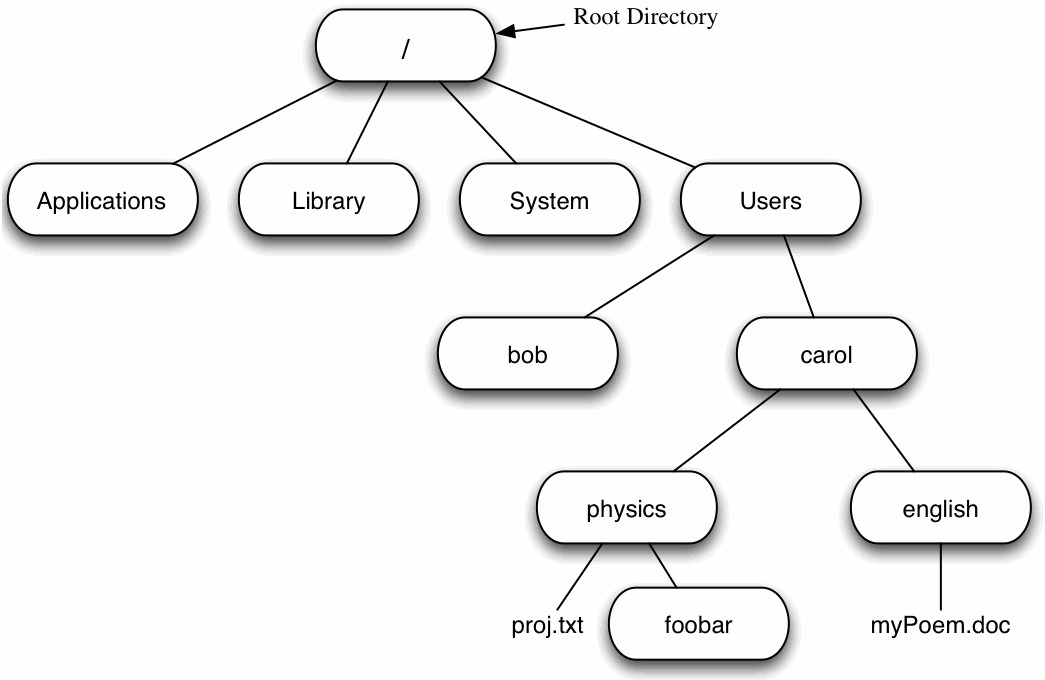
\includegraphics[width=10cm]{./auxfiles/tree.jpg}
\end{figure}


In the diagram above, we see that the home directory of \emph{carol} contains two sub-directories - \emph{physics} and \emph{english}. The full path to the file \emph{myPoem.doc} is \emph{/Users/carol/english/myPoem.doc}. We know that our current working directory \emph{/Users/hautahikingi} is stored inside \emph{Users} because \emph{Users} is the first part of its name. Similarly, we know that \emph{Users} is stored inside the root directory / because its name begins with /. Notice that there are two meanings for the / character. When it appears at the front of a file or directory name, it refers to the root directory. When it appears inside a name, it's just a separator.\\


We can use \emph{cd} followed by a directory name to change our working directory. \emph{cd} stands for \emph{change directory}, which changes the shell's idea of what directory we are in. In the example above, we can type
\begin{lstlisting}
$ cd /users/carol/physics
\end{lstlisting}
\emph{cd} doesn't print anything, but if we run \emph{pwd} after it, we can confirm that the current working directory is \emph{physics}.
\begin{lstlisting}
$ pwd
/users/carol/physics
\end{lstlisting}
If we run \emph{ls} without parameters now, it lists the contents of /users/carol/physics
\begin{lstlisting}
$ ls
proj.txt 	foobar
\end{lstlisting}
We do not have to type the full path to the directory.  Instead, we can use \textbf{relative path references}. When \emph{cd} is followed by a folder path that does not begin with the root directory (/), it assumes that you are first referencing the current working directory. In the above example, because we were located in \emph{/users/carol/} we only needed to type 
\begin{lstlisting}
$ cd physics
\end{lstlisting}
We also do not have to type the entire name of a directory. \emph{Tab Completion} is very handy in situations where the filename is long. Pressing tab asks the terminal to guess what you are trying to type. For example, if we are located in /Users/carol/ and type
\begin{lstlisting}[frame=single]
$ cd ph
\end{lstlisting}
and then press tab, the shell automatically completes the \emph{physics} directory name for us. If, however, there was another directory called \emph{philosophy}. The user would need to type \emph{cd phy} before pressing tab.


\subsection{Creating stuff}
Let's now make a subdirectory called \emph{my\_thesis} which we will work in for this course. I'm going to choose to put it in my Dropbox folder.
\begin{lstlisting}
$ cd Dropbox
$ mkdir my_thesis
$ cd my_thesis
$ pwd
/Users/hautahikingi/Dropbox/my_thesis
\end{lstlisting}
Here, I navigated to the Dropbox folder, made the \emph{my\_thesis} directory, and then navigated into the newly created directory. Let's now create a new file called \emph{draft.txt} using a text editor.
\begin{lstlisting}
$ nano introduction.txt
\end{lstlisting}
I am using \textbf{nano} here because it is the default text editor on a Mac and it is very easy to use. The equivalent on a Windows machine would be \textbf{Notepad}. It's a good idea to become familiar with a more powerful text editor such as Emacs, Vim, SublimeText and Notepad++. Let's type in a few lines of text.
\begin{center}
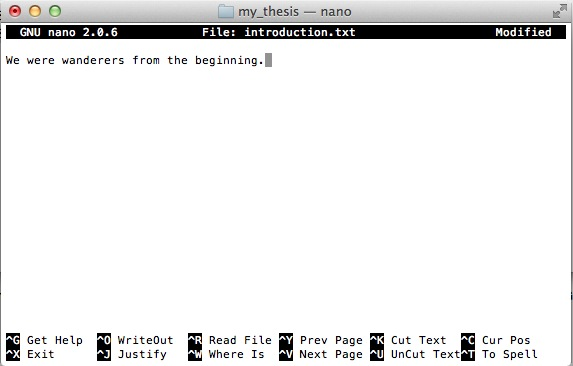
\includegraphics[width=10cm]{./auxfiles/nano.jpg}
\end{center}
In nano, use Control-X to quit the editor and return to the shell. Make sure you save in the process. We can check the changes we've made to a particular file by using the \emph{cat} command. The output of this can get pretty long if we make a lot of changes.
\begin{lstlisting}
$ cat introduction.txt
We were wanderers from the beginning.
\end{lstlisting}
You obviously don't need to create files using the command line. You can do it all the usual way as well. Imagine I just typed up some matlab code which I saved into the my\_thesis folder as \emph{code.m}. Now lets look at:
\begin{lstlisting}
$: ls
code.m	introduction.txt
\end{lstlisting}
We have barely scratched the surface when it comes to things we can do with the terminal command line. There are a ton of online tutorials and textbooks. But for now, we have what we need to move onto Git.

\newpage
\section{Version Control with Git}

Version control is better than mailing files back and forth because:
\begin{itemize}
\item
Nothing that is committed to version control is ever lost. This means it can be used like the \emph{undo} feature in an editor, and since all old versions of files are saved it's always possible to go back in time to see exactly who wrote what on a particular day, or what version of a program was used to generate a particular set of results.
\item
It keeps a record of who made what changes when, so that if people have questions later on, they know who to ask.
\item
It's hard (but not impossible) to accidentally overlook or overwrite someone's changes: the version control system automatically notifies users whenever there's a conflict between one person's work and another's.
\end{itemize}
Git is one of many version control systems. It is more complex than some alternatives, but it is widely used, both because it's easy to set up and because of a hosting site called GitHub, which we will get to later.

\subsection{Set Up}
After downloading Git, an easy way to check if it is installed and working properly is
\begin{lstlisting}
$ git help
\end{lstlisting}
On our first time with Git on a new machine, we need to do a few things. Name, email, clor, editor
\begin{lstlisting}
$ git config --global user.name "Hautahi Kingi"
$ git config --global user.email "hrk55@cornell.edu"
$ git config --global color.ui "auto"
$ git config --global core.editor "nano"
\end{lstlisting}
Navigate to the my\_thesis folder that we created earlier
\begin{lstlisting}
$ cd my_thesis
\end{lstlisting}
and tell git to make it a \emph{repository}. A repository is a storage area where a version control system stores old revisions of files and information about who changed what, when.
\begin{lstlisting}
$ git init
Initialized empty Git repository in /Users/hautahikingi/my_thesis/.git/
\end{lstlisting}
Let's take a look at our new directory
\begin{lstlisting}[frame=single]
$ ls
code.m	introduction.txt
\end{lstlisting}
It looks like nothing has changed. But \emph{ls} does not, in fact, list all the files in the directory, but only those ones whose name does not begin with a dot (.) Files beginning with a dot (.) are known as hidden files and usually contain important program configuration information. They are hidden because you should not change them unless you are very familiar with UNIX.  The \emph{init} command created a hidden directory, and we can see it by using the -a flag
\begin{lstlisting}[frame=single]
$ ls -a
code.m	 .git	introduction.txt
\end{lstlisting}
Git stores information about the project in this special .git sub-directory. If deleted, we lose the project's entire history.\\

An important command is \emph{git status}.
\begin{lstlisting}
$ git status
On branch master

Initial commit

Untracked files:
  (use "git add <file>..." to include in what will be committed)

	code.m
	introduction.txt

nothing added to commit but untracked files present (use "git add" to track)
\end{lstlisting}
While meaningless to a first time user, the output contains a lot of useful information. First of all, it states that we are located on the master branch (more on this later). The \emph{Initial commit} message states that we are yet to make a commit. The \emph{Untracked files} message means that there are files in the directory that Git is not keeping track of.  We tell Git that it should do so using \emph{git add}:
\begin{lstlisting}
$ git add code.m introduction.txt
\end{lstlisting}
and now we check the status again
\begin{lstlisting}
$ git status
On branch master

Initial commit

Changes to be committed:
  (use "git rm --cached <file>..." to unstage)

	new file:   code.m
	new file:   introduction.txt
\end{lstlisting}
This tells us that Git knows that it needs to keep track of the files \emph{code.m} and \emph{introduction.txt}. But it has not yet recorded the changes. To do this we need to \emph{commit}.
\begin{lstlisting}[frame=single]
$ git commit -m "First draft introduction and code"
[master (root-commit) 1ec0eef] First draft introduction and code
 2 files changed, 8 insertions(+)
 create mode 100755 code.m
 create mode 100644 introduction.txt
\end{lstlisting}
Git takes everything we have told it to save by using \emph{git add} and stores a copy permanently inside the special .git directory. This permanent copy has a short identifier 1ec0eef. We use the -m flag to record a comment that will help us remember later on what we did and why. If we just run git commit without the -m option, Git will launch the text editor that you chose at at the start (nano in our case) so that we can write a longer message. Now let's check the status again
\begin{lstlisting}[frame=single]
$ git status
On branch master
nothing to commit, working directory clean
\end{lstlisting}
This is the nice clean message that tells us everything is up to date and committed. It's a good idea to leave the repository in this state before moving onto other work or leaving the office for the weekend.\\

\subsection{Tracking Changes to Files}

Now suppose that after a relaxing weekend, we want to launch back into work. I've created a latex file called template.tex.
\begin{lstlisting}
$ ls
code.m              template.aux        template.pdf        template.tex
draft.txt           template.log        template.synctex.gz
\end{lstlisting}
We can see that my particular latex compiler created a number of auxiliary files. Checking the status of the repository gives
\begin{lstlisting}
$ git status
On branch master
Untracked files:
  (use "git add <file>..." to include in what will be committed)

	template.aux
	template.log
	template.pdf
	template.synctex.gz
	template.tex

nothing added to commit but untracked files present (use "git add" to track)
\end{lstlisting}
This tells us that there are new files that have been created which Git has not been instructed to keep a track of. I don't particularly care about the auxiliary latex files so putting them under version control would be a waste of disk space. What's worse, having them all listed could distract us from changes that actually matter, so let's tell Git to ignore them. We do this by creating a file in the root directory of our project called .gitignore.
\begin{lstlisting}
$ nano .gitignore
\end{lstlisting}
\begin{center}
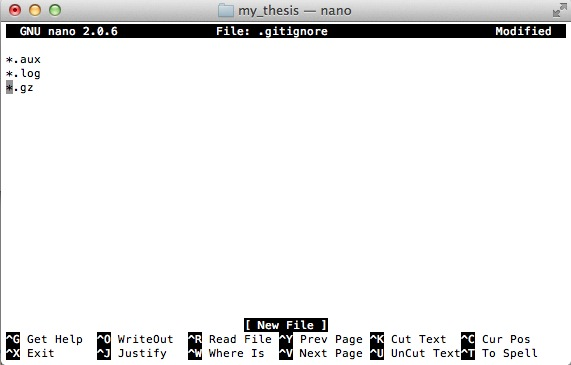
\includegraphics[width=10cm]{./auxfiles/gitignore.jpg}
\end{center}
We've told Git to ignore any file whose name ends in .aux, .log and .gz. Once we have created this file, the output of git status is much cleaner:
\begin{lstlisting}
$ git status
On branch master
Untracked files:
  (use "git add <file>..." to include in what will be committed)

	.gitignore
	template.pdf
	template.tex

nothing added to commit but untracked files present (use "git add" to track)
\end{lstlisting}
The only thing Git notices now is the newly-created .gitignore file. You might think we wouldn't want to track it, but everyone we're sharing our repository with will probably want to ignore the same things that we're ignoring.\\


Now let's make one more edit to our code.m file and check the status again.
\begin{lstlisting}
$ git status
\end{lstlisting}
\begin{lstlisting}
On branch master
Changes not staged for commit:
  (use "git add <file>..." to update what will be committed)
  (use "git checkout -- <file>..." to discard changes in working directory)

	modified:   code.m

Untracked files:
  (use "git add <file>..." to include in what will be committed)

	.gitignore
	template.pdf
	template.tex

no changes added to commit (use "git add" and/or "git commit -a")
\end{lstlisting}
As well as the issue with the latex file in the previous status check, git also tells us that the code.m file has been modified. Let's now add and commit these changes.
\begin{lstlisting}[frame=single]
$ git add code.m template.tex template.pdf .gitignore
$ git status
On branch master
Changes to be committed:
  (use "git reset HEAD <file>..." to unstage)

	modified:   code.m
	new file:   template.tex
$ git commit -m "New latex file and change to code.m"
[master 170ae6f] New latex file and change to code.m
 4 files changed, 49 insertions(+)
 create mode 100644 .gitignore
 create mode 100644 template.pdf
 create mode 100644 template.tex
\end{lstlisting}
and checking the status....
\begin{lstlisting}[frame=single]
$ git status
\end{lstlisting}
\begin{lstlisting}[frame=single]
On branch master
nothing to commit, working directory clean
\end{lstlisting}
... we're back to a clean sheet.\\

\subsection{The Git Cycle}
We should now be able to see the basic structure of how Git works. Once a directory is set up as a Git repository using \emph{git init}, any change that we make to that directory is noted by Git. The workflow is then as follows:
\begin{enumerate}
\item
Modify/create new folders and files.
\item
Stage these changes ready to commit by using \emph{git add}.
\item
Commit the changes using \emph{git commit} which permanently saves the current version of that repository.
\end{enumerate}

\newpage
\section{GitHub: Taking Version Control Online}

Version control really comes into its own when we begin to collaborate with other people. In practice, groups like to use a central hub/cloud stored on the web rather than on someone's laptop so that all collaborators can easily access the repository. Git is so popular because of websites like Github and BitBucket which make collaboration so easy.\\

Login to your profile page on GitHub. Click on the icon in the top right corner to create a new repository called my\_thesis.
\begin{center}
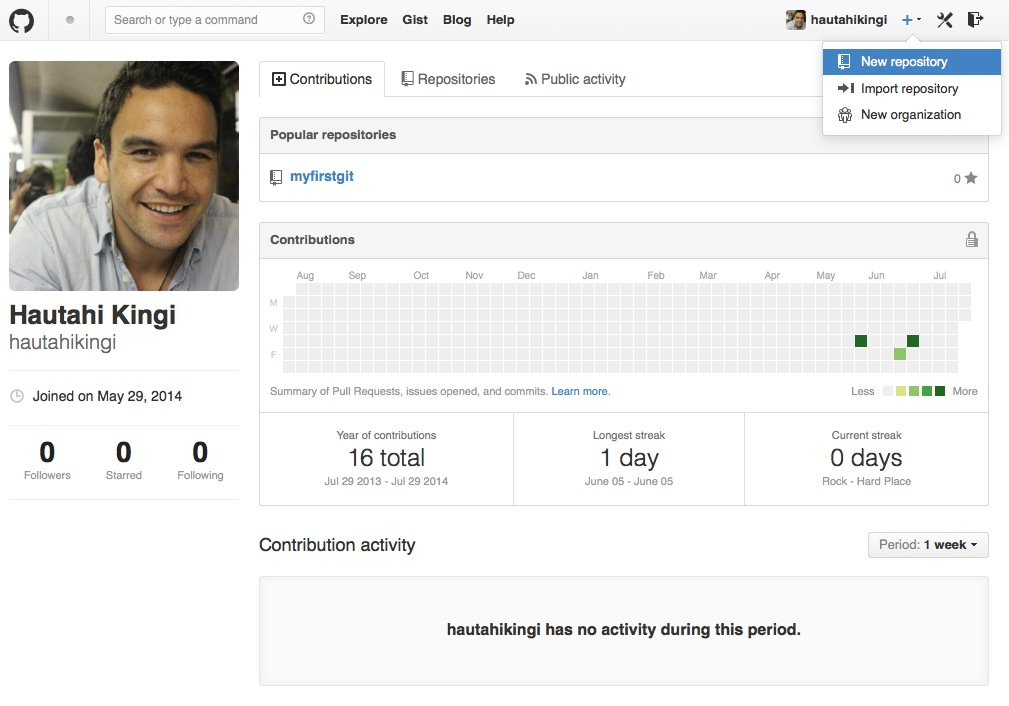
\includegraphics[width=10cm]{./auxfiles/Ghub.jpg}
\end{center}

If you wish, you can enter a description but this is not necessary. You can also choose the privacy settings of your repository. Public repositories allow any Github user to access your files. A student account receives 5 free private repositories.

\begin{center}
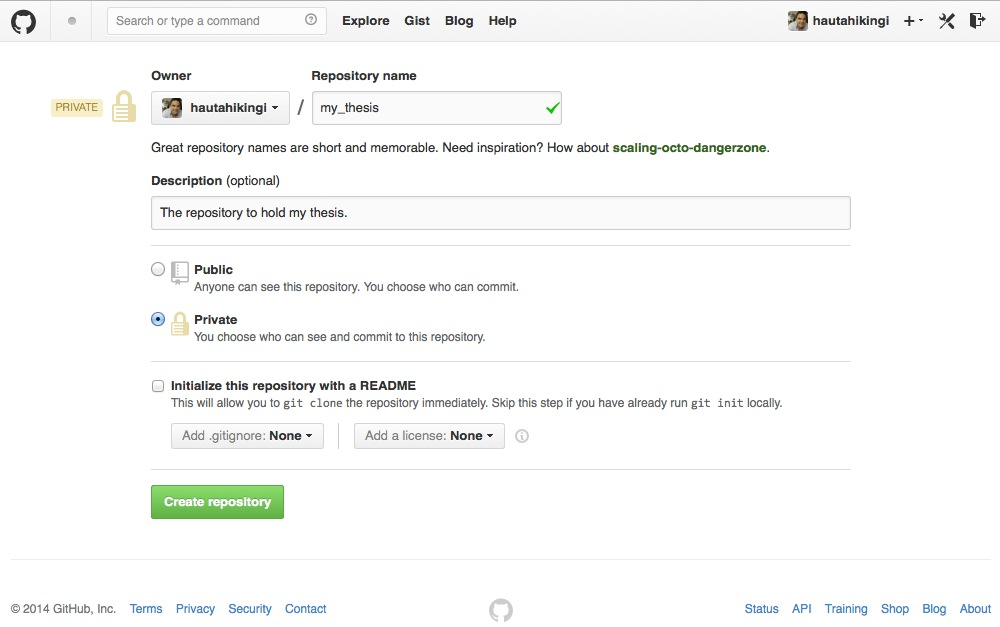
\includegraphics[width=10cm]{./auxfiles/Ghub1.jpg}
\end{center}

Clicking the green button creates a repository on the Github website. As soon as the repository is created, GitHub displays a page with a URL and some information on how to configure your local repository. 

\begin{center}
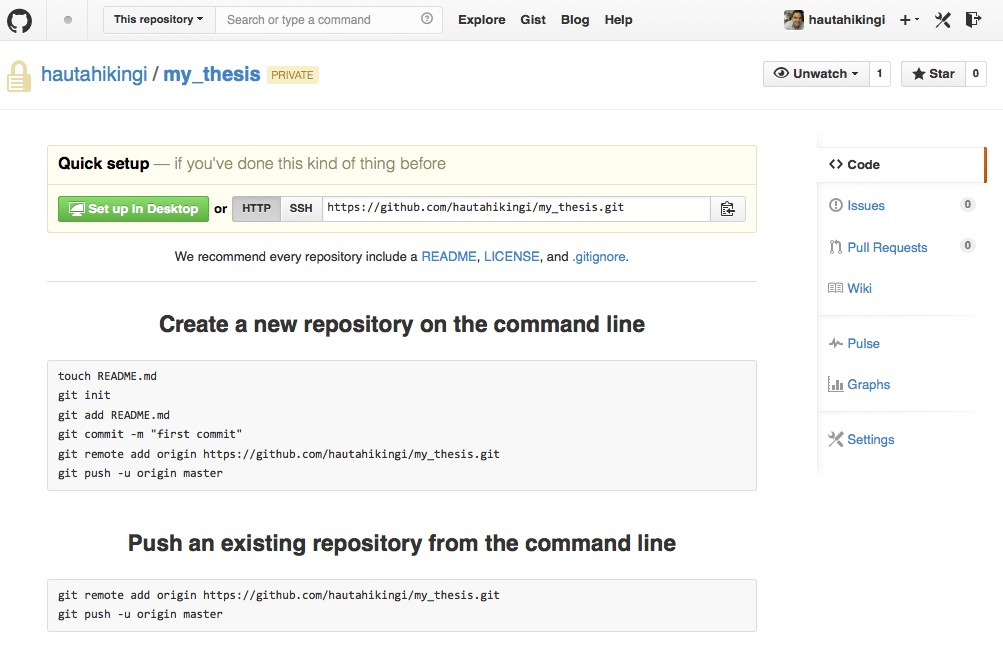
\includegraphics[width=10cm]{./auxfiles/Ghub2.jpg}
\end{center}

Remember, our local repository still contains our earlier work, but the remote repository on GitHub doesn't contain any files yet. The next step is to connect the two repositories. We do this by making the GitHub repository a remote for the local repository. The home page of the repository on GitHub includes the string we need to identify it. Since we have already created a repository on our local computer, we are interested in the instructions in the second box. Making sure we are in the my\_thesis directory locally...
\begin{lstlisting}[frame=single]
$ git remote add origin https://github.com/hautahikingi/my_thesis.git
\end{lstlisting}
This command tells git to add a remote named \emph{origin} at the url \emph{https://github.com/hautahikingi/my\_thesis.git}. \emph{origin} is a nickname we've assigned to the particular remote repository. We could have called it anything but origin is the most common choice. We can check that the command worked by typing
\begin{lstlisting}[frame=single]
$ git remote -v
\end{lstlisting}
\begin{lstlisting}[frame=single]
origin	https://github.com/hautahikingi/my_thesis.git (fetch)
origin	https://github.com/hautahikingi/my_thesis.git (push)
\end{lstlisting}

which lists all remote repositories. The -v flag is short for verbose which tells git to show the remote url as well as the nickname.\\

Note that so far all we have done is set up a remote repository and linked it to our local repository. But if we take a look at our remote repository, it is still empty. We fix this by pushing the changes from our local repository to the repository on GitHub
\begin{lstlisting}
$ git push origin master
\end{lstlisting}
It will sometimes ask for your username and password
\begin{lstlisting}[frame=single]
Username for 'https://github.com': hautahikingi
Password for 'https://hautahikingi@github.com':
\end{lstlisting}
When you are typing in your password the cursor won't move. Don't panic just type it out and press enter.
\begin{lstlisting}[frame=single]
Counting objects: 10, done.
Delta compression using up to 4 threads.
Compressing objects: 100\% (8/8), done.
Writing objects: 100\% (10/10), 42.65 KiB | 0 bytes/s, done.
Total 10 (delta 1), reused 0 (delta 0)
To https://github.com/hautahikingi/my_thesis.git
 * [new branch]      master -> master
Branch master set up to track remote branch master from origin.
\end{lstlisting}

Our local and remote repositories are now synced. Let's now look at the website. We can see the files reflected in it.\\

\begin{center}
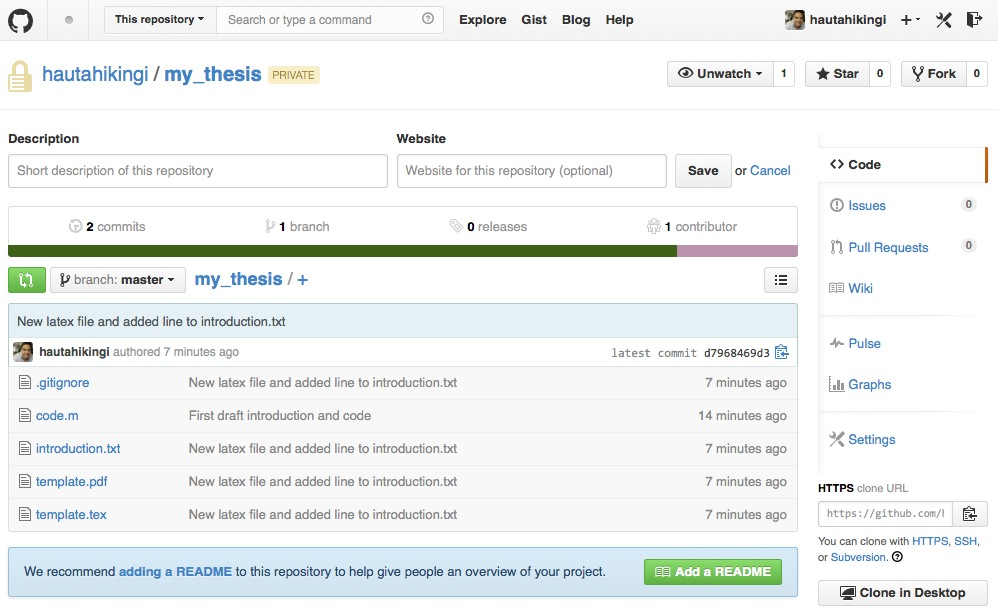
\includegraphics[width=10cm]{./auxfiles/Ghub3.jpg}
\end{center}

If we go to the graphs tab on the right of the GitHub page, we can take a look at the network.

\begin{center}
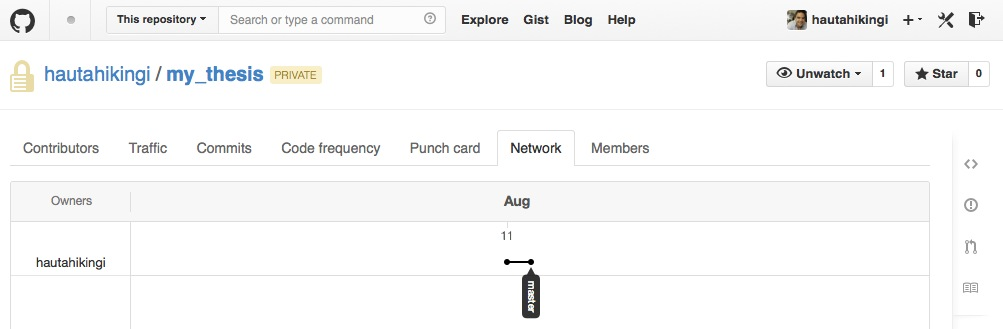
\includegraphics[width=10cm]{./auxfiles/Network.jpg}
\end{center}

This gives a visual representation of the evolution of the repository. Each commit is represented by a node in the graph. There are two nodes here because we have performed two commits. Note that even though we have only pushed our local copy to the remote repository once, GitHub shows each commit that has occured. This is one of the main advantages of Git over other version control systems such as Subversion, which only records commits that are made directly to the remote repository. So for example, in subversion, there would only be one node in this tree. This is what people mean when they speak of \textbf{centralized} vs \textbf{distributed} version control.\\

A more complicated network map looks like...\\

\begin{center}
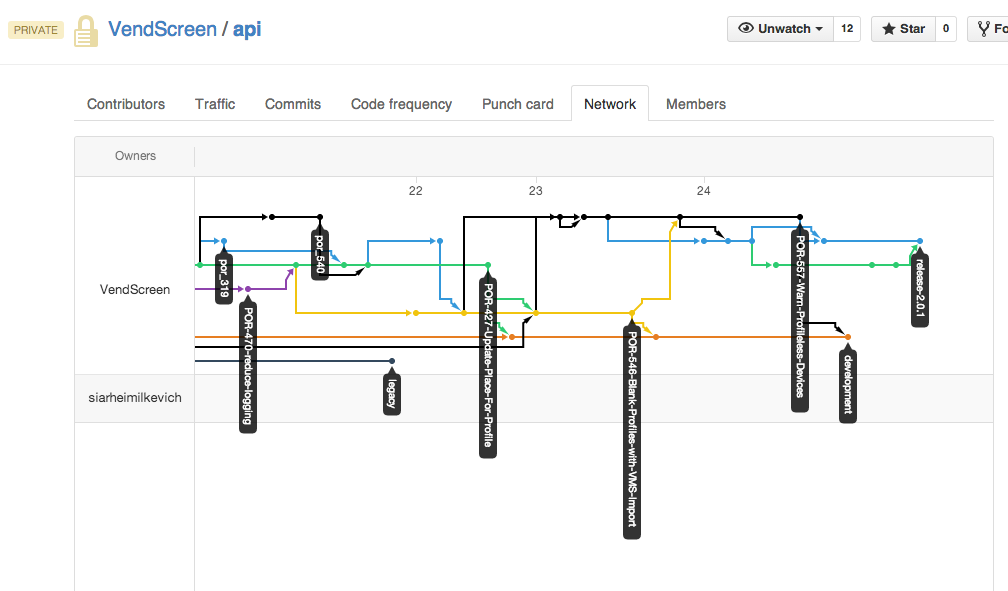
\includegraphics[width=10cm]{./auxfiles/network_comp.png}
\end{center}

We can pull changes from the remote repository to the local one as well:

\begin{lstlisting}[frame=single]
$ git pull origin master
From https://github.com/hautahikingi/my_thesis
 * branch            master     -> FETCH_HEAD
Already up-to-date.
\end{lstlisting}
Pulling has no effect in this case because the two repositories are already synchronized. If someone else had pushed some changes to the repository on GitHub, though, this command would download them to our local repository.\\

Let's now do a tricky exercise. We can simulate working with a collaborator using another copy of the repository on our local machine. To do this, \emph{cd} to another directory on your computer. Instead of creating a new repository here with git init, we will clone the existing repository from GitHub.\\

\begin{lstlisting}
$ cd /Users/hautahikingi/Dropbox/temporary
$ git clone https://github.com/hautahikingi/my_thesis.git
Cloning into 'my_thesis'...
remote: Counting objects: 10, done.
remote: Compressing objects: 100\% (7/7), done.
remote: Total 10 (delta 1), reused 10 (delta 1)
Unpacking objects: 100\% (10/10), done.
Checking connectivity... done.
\end{lstlisting}
Here, I navigated to a new folder called \emph{temporary}. I then created a fresh local copy of a remote repository. (We did it in /temporary or some other directory so that we don't overwrite our existing my\_thesis directory.) Our computer now has two copies of the repository. One in \emph{/Users/hautahikingi/Dropbox/temporary} and one in \emph{/Users/hautahikingi/Dropbox/}. Let's make a change to the copy in \emph{/temporary/my\_thesis}:
\begin{lstlisting}
$ nano introduction.txt
$ cat introduction.txt
We were wanderers from the beginning.
We knew every stand of tree for a hundred miles.
\end{lstlisting}
and now let's add and commit
\begin{lstlisting}
$ git add introduction.txt
$ git commit -m "Added a second line to introduction.txt"
\end{lstlisting}
and checking the status..
\begin{lstlisting}
$ git status
On branch master
Your branch is ahead of 'origin/master' by 1 commit.
  (use "git push" to publish your local commits)

nothing to commit, working directory clean
\end{lstlisting}
This message tells us that we have committed all changes, but that we have not yet pushed these changes to the remote repository on Github. Again, this can only be done on \textbf{distributed} version control systems.\\

Let's now push the change to Github
\begin{lstlisting}
$ git push origin master
Counting objects: 5, done.
Delta compression using up to 4 threads.
Compressing objects: 100\% (3/3), done.
Writing objects: 100\% (3/3), 345 bytes | 0 bytes/s, done.
Total 3 (delta 1), reused 0 (delta 0)
To https://github.com/hautahikingi/my_thesis.git
   170ae6f..3cafe3a  master -> master
\end{lstlisting}
Checking the status...
\begin{lstlisting}
$ git status
On branch master
Your branch is up-to-date with 'origin/master'.

nothing to commit, working directory clean
\end{lstlisting}
This tells us that we have committed all changes, and that this is also reflected in the remote repository. The network map also confirms this...
\begin{center}
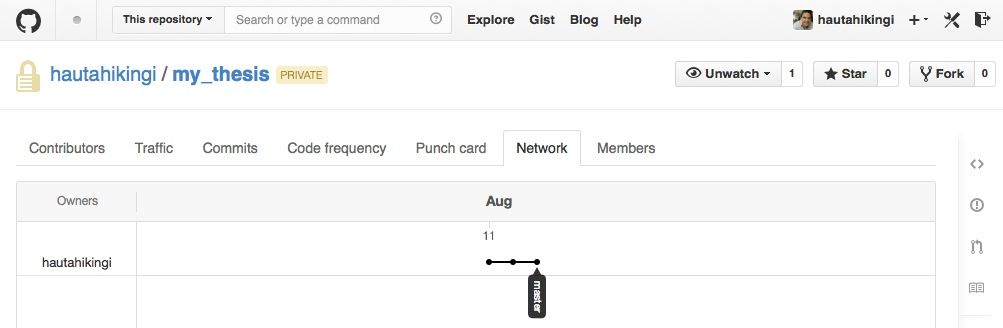
\includegraphics[width=10cm]{./auxfiles/Network_update.jpg}
\end{center}
We can now download changes into the original repository on our machine:
\begin{lstlisting}
$ cd /Users/hautahikingi/Dropbox/my_thesis
$ git pull origin master
\end{lstlisting}
so that both our local repositories are now in sync with the remote repository. In practice, we would probably never have two copies of the same remote repository on our laptop at once. Instead, one of those copies would be on our laptop, and the other on a lab machine, or on someone else's computer. Pushing and pulling changes gives us a reliable way to share work between different people and machines


\subsection{The GitHub GUI}

There are now a number of fantastic GUIs which work well with Github. Let's take a quick look at the GUI created by Github itself.

When we first launch the GUI we want to tell it to add our local repository from the menu.
\begin{center}
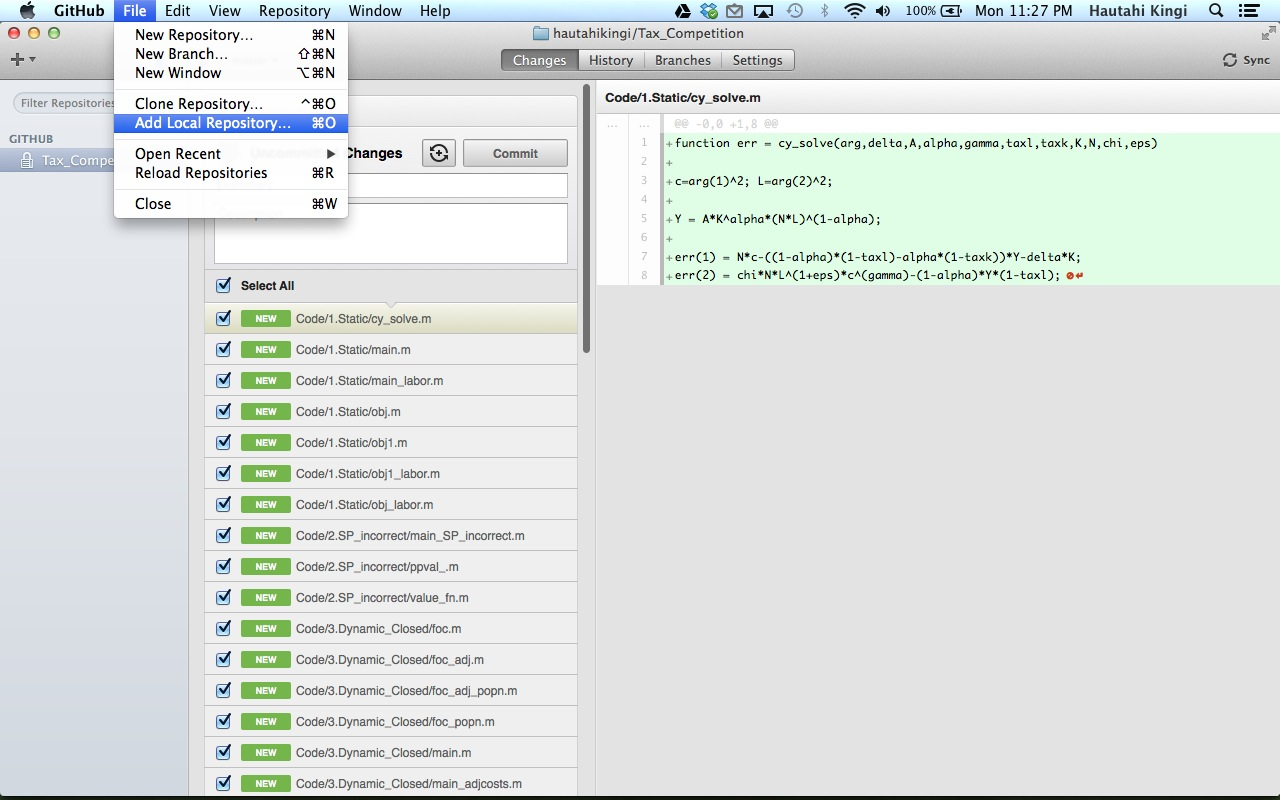
\includegraphics[width=10cm]{./auxfiles/GUI_add.jpg}
\end{center}
After then selecting the repository in the left-hand menu, the right hand pane shows a range of information about that repository contained in four separate panels.
\begin{center}
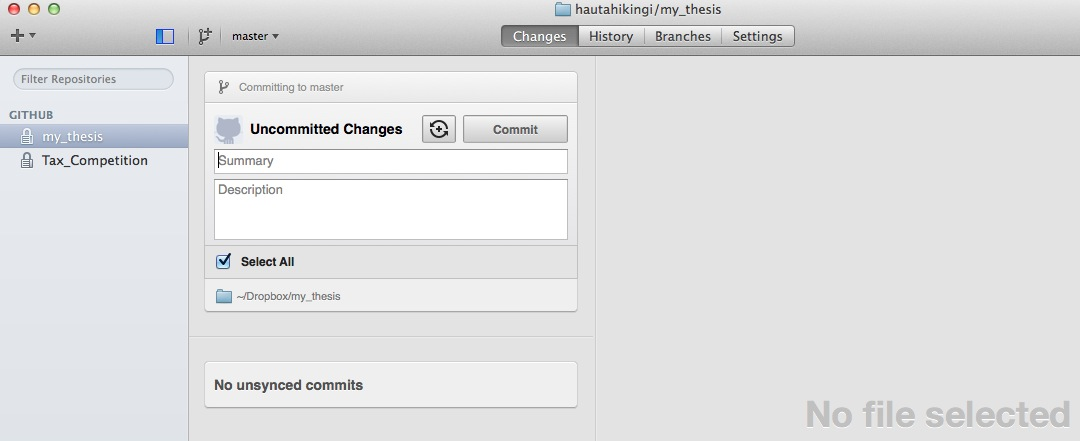
\includegraphics[width=10cm]{./auxfiles/GUI_changes.jpg}
\end{center}
The \emph{changes} panel shows the changes made within the repository which are yet to be committed. It effectively shows the same information as typing \emph{git status} in the command line. As you can see, we have nothing untracked or changed since the last commit.
\begin{center}
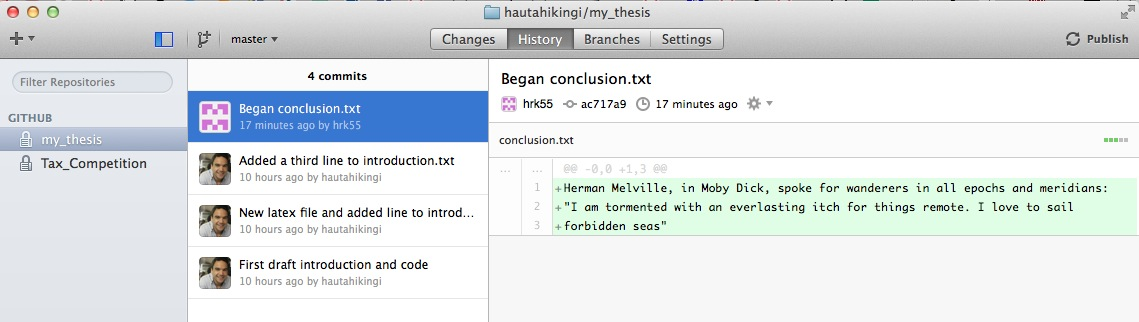
\includegraphics[width=10cm]{./auxfiles/GUI_history.jpg}
\end{center}
The history panel allows us to select each commit, and investigate what changes were made since the last commit.\\


%\section{Exercises}
%
%What do ls ~ and ls ~/.. list?


For a far more comprehensive coverage of the topics covered in this mini-course, please refer to the Software carpentry website mentioned at the beginning of these notes.
\end{document}
